\documentclass[border=10pt]{standalone}
\usepackage{tikz}\usepackage{amsmath}\usetikzlibrary{arrows.meta,patterns}
\begin{document}
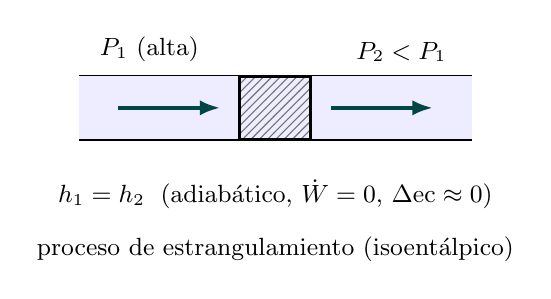
\begin{tikzpicture}[line width=1pt,>={Latex[length=2.6mm]}]
  % tuberia
  \draw[line width=1.2pt] (-2.5,0.4)--(2.5,0.4) (-2.5,-0.4)--(2.5,-0.4);
  \fill[blue!7] (-2.5,-0.4) rectangle (2.5,0.4);
  % tapon poroso (estrangulamiento)
  \fill[pattern=north east lines,pattern color=black!55] (-0.45,-0.4) rectangle (0.45,0.4);
  \draw[line width=1.1pt] (-0.45,-0.4) rectangle (0.45,0.4);
  % flujo
  \draw[->,teal!55!black,line width=1.4pt] (-2.0,0)--(-0.7,0);
  \draw[->,teal!55!black,line width=1.4pt] (0.7,0)--(2.0,0);
  \node[above] at (-1.6,0.45){\small $P_1$ (alta)};
  \node[above] at (1.6,0.45){\small $P_2<P_1$};
  \node at (0,-1.1){\small $h_1=h_2$ \;(adiabático, $\dot W=0$, $\Delta\mathrm{ec}\approx0$)};
  \node at (0,-1.8){\small proceso de estrangulamiento (isoentálpico)};
\end{tikzpicture}
\end{document}
